\begin{figure}[!htb] % Two node transitive
\centering
\begin{minipage}{1.2in}
\begin{tikzpicture}[node distance=3cm]
\node [roundnode] (a) {a};
\node [roundnode] (b) [right of=a] {b};
\draw[ultra thick, ->] (b) -- (a);
\end{tikzpicture}
\end{minipage}
\hfill
\begin{minipage}{1.2in}
\[
M=
  \begin{bmatrix}
    1 & 0 \\
    1 & 0 \\
  \end{bmatrix}
\]
\end{minipage}
\hfill
\begin{minipage}{1.2in}
\begin{tikzpicture}
\def\v{2}
\def\x{2} % 2 * 1
\coordinate (O) at (0,0);
\coordinate (X) at (\x,0);
\draw [->] (O) -- (\v,0) node[below]{$x$};
\draw [->] (O) -- (0,\v) node[left]{$y$};
\draw [ultra thick, ->] (O) -- (X) node[right]{$v_1$};
\end{tikzpicture}
\end{minipage}
\caption{Preference graph $G$, transition matrix $M$, and principal eigenvector $v_1$ for a two-node transitive preference. $||v_1||_2^2 = 1$, $H_T(G) = 0$. Steady state achieved after one iteration.}
\label{fig:linalg_1} 
\end{figure}



\begin{figure}[!htb] % Two node cycle
\centering
\begin{minipage}{1.2in}
\begin{tikzpicture}[node distance=3cm]
\node [roundnode] (a) {a};
\node [roundnode] (b) [right of=a] {b};
\draw[ultra thick, ->] (b) to[bend right] (a);
\draw[ultra thick, ->] (a) to[bend right] (b);
\end{tikzpicture}
\end{minipage}
\hfill
\begin{minipage}{1.2in}
\[
M=
  \begin{bmatrix}
    .5 & .5 \\
    .5 & .5 \\
  \end{bmatrix}
\]
\end{minipage}
\hfill
\begin{minipage}{1.2in}
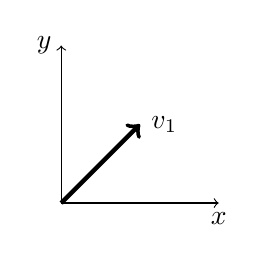
\begin{tikzpicture}
\def\v{2}
\def\x{1} % 2 * .5
\coordinate (O) at (0,0);
\coordinate (X) at (\x,\x);
\draw [->] (O) -- (\v,0) node[below]{$x$};
\draw [->] (O) -- (0,\v) node[left]{$y$};
\draw [ultra thick, ->] (O) -- (X) node[right]{$v_1$};
\end{tikzpicture}
\end{minipage}
\caption{Preference graph $G$, transition matrix $M$, and principal eigenvector $v_1$ for a two-node cycle. $||v_1||_2^2 = 1/2$, $H_T(G) = 1$. Intuitively, we set the probability of each item equal to the average of the prior preferences. The normalizing restriction on $v$ ensures that these averages continue to represent a distribution over the items. Note also that the steady state (a uniform distribution) is achieved after only one iteration.}
\label{fig:linalg_2} 
\end{figure}



\begin{figure}[!htb] % Three node transitive
\centering
\begin{minipage}{1.2in}
\begin{tikzpicture}[node distance=3cm]
\node [roundnode] (a) {a};
\node [roundnode] (b) [right of=a] {b};
\node [roundnode] (c) [below of=a] {c};
\draw[ultra thick, ->] (b) -- (a);
\draw[ultra thick, ->] (c) -- (b);
\draw[ultra thick, ->] (c) -- (a);
\end{tikzpicture}
\end{minipage}
\hfill
\begin{minipage}{1.2in}
\[
M=
  \begin{bmatrix}
    1 & 0 & 0 \\
    .5 & .5 & 0 \\
    .5 & .5 & 0
  \end{bmatrix}
\]
\end{minipage}
\hfill
\begin{minipage}{1.2in}
\begin{tikzpicture}
\def\v{2}
\def\x{2} % 2 * 1
\coordinate (O) at (0,0,0);
\coordinate (X) at (\x,0,0);
\draw [->] (O) -- (\v,0,0) node[below]{$x$};
\draw [->] (O) -- (0,\v,0) node[left]{$z$};
\draw [->] (O) -- (0,0,\v) node[below]{$y$};
\draw [ultra thick, ->] (O) -- (X) node[right]{$v_1$};
\end{tikzpicture}
\end{minipage}
\caption{Preference graph $G$, transition matrix $M$, and principal eigenvector $v_1$ for a three-node transitive preference. $||v_1||_2^2 = 1$, $H_T(G) = 0.918$. In this case, the steady state is achieved in the limit. At every iteration, C sends its probability mass to A and B evenly, and has no mass after the first iteration. B splits its mass between itself and A, while A directs all of its mass towards itself. The limiting convergence is due to the logarithmic reallocation of mass from B to A (a bit of a Zeno-style paradox).}
\label{fig:linalg_3} 
\end{figure}



\begin{figure}[!htb] % Three node cycle
\centering
\begin{minipage}{1.2in}
\begin{tikzpicture}[node distance=3cm]
\node [roundnode] (a) {a};
\node [roundnode] (b) [right of=a] {b};
\node [roundnode] (c) [below of=a] {c};
\draw[ultra thick, ->] (b) -- (a);
\draw[ultra thick, ->] (c) -- (b);
\draw[ultra thick, ->] (a) -- (c);
\end{tikzpicture}
\end{minipage}
\hfill
\begin{minipage}{1.2in}
\[
M=
  \begin{bmatrix}
    .5 & 0 & .5 \\
    .5 & .5 & 0 \\
    0 & .5 & .5
  \end{bmatrix}
\]
\end{minipage}
\hfill
\begin{minipage}{1.2in}
\begin{tikzpicture}
\def\v{2}
\def\x{.66} % 2 * 1/3
\coordinate (O) at (0,0,0);
\coordinate (X) at (\x,\x,\x);
\coordinate (Xxy) at (\x,0,\x);
\draw [->] (O) -- (\v,0,0) node[below]{$x$};
\draw [->] (O) -- (0,\v,0) node[left]{$z$};
\draw [->] (O) -- (0,0,\v) node[below]{$y$};
\draw [ultra thick, ->] (O) -- (X) node[right]{$v_1$};
\draw [dashed, color=red] (O) -- (Xxy);
\draw [dashed, color=red] (X) -- (Xxy);
\end{tikzpicture}
\end{minipage}
\caption{Preference graph $G$, transition matrix $M$, and principal eigenvector $v_1$ for a three-node cycle. $||v_1||_2^2 = 1/3$, $H_T(G) = 1.585$. Here the reallocation of probability mass across iterations exhibits more complex dynamics, and converges to $v_1$ in the limit.}
\label{fig:linalg_4} 
\end{figure}



\begin{figure}[!htb] % Three node double cycle
\centering
\begin{minipage}{1.2in}
\begin{tikzpicture}[node distance=3cm]
\node [roundnode] (a) {a};
\node [roundnode] (b) [right of=a] {b};
\node [roundnode] (c) [below of=a] {c};
\draw[ultra thick, ->] (b) to[bend right] (a);
\draw[ultra thick, ->] (c) to[bend right] (b);
\draw[ultra thick, ->] (a) to[bend right] (c);
\draw[ultra thick, ->] (a) -- (b);
\draw[ultra thick, ->] (b) -- (c);
\draw[ultra thick, ->] (c) -- (a);
\end{tikzpicture}
\end{minipage}
\hfill
\begin{minipage}{1.2in}
\[
M=
  \begin{bmatrix}
    .5 & .25 & .25 \\
    .25 & .5 & .25 \\
    .25 & .25 & .5
  \end{bmatrix}
\]
\end{minipage}
\hfill
\begin{minipage}{1.2in}
\begin{tikzpicture}
\def\v{2}
\def\x{.66} % 2 * 1/3
\coordinate (O) at (0,0,0);
\coordinate (X) at (\x,\x,\x);
\coordinate (Xxy) at (\x,0,\x);
\draw [->] (O) -- (\v,0,0) node[below]{$x$};
\draw [->] (O) -- (0,\v,0) node[left]{$z$};
\draw [->] (O) -- (0,0,\v) node[below]{$y$};
\draw [ultra thick, ->] (O) -- (X) node[right]{$v_1$};
\draw [dashed, color=red] (O) -- (Xxy);
\draw [dashed, color=red] (X) -- (Xxy);
\end{tikzpicture}
\end{minipage}
\caption{Preference graph $G$, transition matrix $M$, and principal eigenvector $v_1$ for a three-node double cycle. $||v_1||_2^2 = 1/3$, $H_T(G) = 1.585$}
\label{fig:linalg_5} 
\end{figure}



\begin{figure}[!htb] % Three node transitive with edge weights
\centering
\begin{minipage}{1.2in}
\begin{tikzpicture}[node distance=3cm]
\node [roundnode] (a) {a};
\node [roundnode] (b) [right of=a] {b};
\node [roundnode] (c) [below of=a] {c};
\draw[ultra thick, ->] (a) -- node[auto] {1} (b);
\draw[ultra thick, ->] (b) -- node[auto] {1} (c);
\draw[ultra thick, ->] (c) -- node[auto] {3} (a);
\end{tikzpicture}
\end{minipage}
\hfill
\begin{minipage}{1.2in}
\[
M=
  \begin{bmatrix}
    .75 & .25 & 0 \\
    0 & .5 & .5 \\
    .75 & 0 & .25
  \end{bmatrix}
\]
\end{minipage}
\hfill
\begin{minipage}{1.2in}
\begin{tikzpicture}
\def\v{2}
\def\a{1.09068489}
\def\b{0.54557228}
\def\c{0.36374283}
\coordinate (O) at (0,0,0);
\coordinate (X) at (\a,\c,\b);
\coordinate (Xxy) at (\a,0,\b);
\draw [->] (O) -- (\v,0,0) node[below]{$x$};
\draw [->] (O) -- (0,\v,0) node[left]{$z$};
\draw [->] (O) -- (0,0,\v) node[below]{$y$};
\draw [ultra thick, ->] (O) -- (X) node[right]{$v_1$};
\draw [dashed, color=red] (O) -- (Xxy);
\draw [dashed, color=red] (X) -- (Xxy);
\end{tikzpicture}
\end{minipage}
\caption{Preference graph $G$, transition matrix $M$, and principal eigenvector $v_1$ for a three-node cycle with edge weights. $||v_1||_2^2 = 0.4049$, $H_T(G) = 1.371$. Note how the introduction of variable weights repositions $v_1$ within the simplex, allowing us to recover a transitive ordering $a > b > c$.}
\label{fig:linalg_6} 
\end{figure}


\begin{figure}[!htb] % Four node two cycle
\centering
\begin{minipage}{1.2in}
\begin{tikzpicture}[node distance=3cm]
\node [roundnode] (a) {a};
\node [roundnode] (b) [right of=a] {b};
\node [roundnode] (c) [below of=a] {c};
\node [roundnode] (d) [below of=b] {d};
\draw[ultra thick, ->] (a) -- (c);
\draw[ultra thick, ->] (b) -- (a);
\draw[ultra thick, ->] (c) -- (b);
\draw[ultra thick, ->] (d) -- (a);
\draw[ultra thick, ->] (d) -- (b);
\draw[ultra thick, ->] (c) -- (d);
\end{tikzpicture}
\end{minipage}
\hfill
\begin{minipage}{1.2in}
\[
M=
  \begin{bmatrix}
    .66 & 0 & .33 & 0 \\
    .33 & .66 & 0 & 0 \\
    0 & .33 & .33 & .33 \\
    .33 & .33 & 0 & .33
  \end{bmatrix}
\]
\end{minipage}
\hfill
\begin{minipage}{1.2in}
\[
(.4, .3, .2, .1)
\]
\end{minipage}
\caption{Preference graph $G$, transition matrix $M$, and principal eigenvector $v_1$ for a four-node graph with two cycles. $||v_1||_2^2 = 0.3$, $H_T(G) = 1.918$.}
\label{fig:linalg_7} 
\end{figure}


\begin{figure}[!htb] % Four node upper cycle
\centering
\begin{minipage}{1.2in}
\begin{tikzpicture}[node distance=3cm]
\node [roundnode] (a) {a};
\node [roundnode] (b) [right of=a] {b};
\node [roundnode] (c) [below of=a] {c};
\node [roundnode] (d) [below of=b] {d};
\draw[ultra thick, ->] (a) -- (c);
\draw[ultra thick, ->] (c) -- (b);
\draw[ultra thick, ->] (b) -- (a);
\draw[ultra thick, ->] (d) -- (a);
\draw[ultra thick, ->] (d) -- (b);
\draw[ultra thick, ->] (d) -- (c);
\end{tikzpicture}
\end{minipage}
\hfill
\begin{minipage}{1.2in}
\[
M=
  \begin{bmatrix}
    .66 & 0 & .33 & 0 \\
    .33 & .66 & 0 & 0 \\
    0 & .33 & .66 & 0 \\
    .33 & .33 & .33 & 0
  \end{bmatrix}
\]
\end{minipage}
\hfill
\begin{minipage}{1.2in}
\[
(.33, .33, .33, 0)
\]
\end{minipage}
\caption{Preference graph $G$, transition matrix $M$, and principal eigenvector $v_1$ for a four-node graph with one cycle. $||v_1||_2^2 = 1/3$, $H_T(G) = 1.585$. Note that we see a cycle in $v_1$, despite having a larger $L_2$ value than the previous example.}
\label{fig:linalg_8} 
\end{figure}


\begin{figure}[!htb] % Four node lower cycle
\centering
\begin{minipage}{1.2in}
\begin{tikzpicture}[node distance=3cm]
\node [roundnode] (a) {a};
\node [roundnode] (b) [right of=a] {b};
\node [roundnode] (c) [below of=a] {c};
\node [roundnode] (d) [below of=b] {d};
\draw[ultra thick, ->] (b) -- (a);
\draw[ultra thick, ->] (c) -- (a);
\draw[ultra thick, ->] (d) -- (a);
\draw[ultra thick, ->] (b) -- (c);
\draw[ultra thick, ->] (c) -- (d);
\draw[ultra thick, ->] (d) -- (b);
\end{tikzpicture}
\end{minipage}
\hfill
\begin{minipage}{1.2in}
\[
M=
  \begin{bmatrix}
    1 & 0 & 0 & 0 \\
    .33 & .33 & .33 & 0 \\
    .33 & 0 & .33 & .33 \\
    .33 & .33 & 0 & .33
  \end{bmatrix}
\]
\end{minipage}
\hfill
\begin{minipage}{1.2in}
\[
(1, 0, 0, 0)
\]
\end{minipage}
\caption{Preference graph $G$, transition matrix $M$, and principal eigenvector $v_1$ for a four-node graph with one cycle. $||v_1||_2^2 = 1$, $H_T(G) = 1.793$. Note how the presence of a cycle in the lower nodes does not prevent the graph from having high level of structure.}
\label{fig:linalg_9} 
\end{figure}